\documentclass[11pt,ignorenonframetext,]{beamer}
\setbeamertemplate{caption}[numbered]
\setbeamertemplate{caption label separator}{: }
\setbeamercolor{caption name}{fg=normal text.fg}
\beamertemplatenavigationsymbolsempty
\usepackage{lmodern}
\usepackage{amssymb,amsmath}
\usepackage{ifxetex,ifluatex}
\usepackage{fixltx2e} % provides \textsubscript
\ifnum 0\ifxetex 1\fi\ifluatex 1\fi=0 % if pdftex
  \usepackage[T1]{fontenc}
  \usepackage[utf8]{inputenc}
\else % if luatex or xelatex
  \ifxetex
    \usepackage{mathspec}
  \else
    \usepackage{fontspec}
  \fi
  \defaultfontfeatures{Ligatures=TeX,Scale=MatchLowercase}
\fi
\usetheme[]{metropolis}
% use upquote if available, for straight quotes in verbatim environments
\IfFileExists{upquote.sty}{\usepackage{upquote}}{}
% use microtype if available
\IfFileExists{microtype.sty}{%
\usepackage{microtype}
\UseMicrotypeSet[protrusion]{basicmath} % disable protrusion for tt fonts
}{}
\newif\ifbibliography
\hypersetup{
            pdftitle={Lecture 21},
            pdfauthor={Colin Rundel},
            pdfborder={0 0 0},
            breaklinks=true}
\urlstyle{same}  % don't use monospace font for urls
\usepackage{color}
\usepackage{fancyvrb}
\newcommand{\VerbBar}{|}
\newcommand{\VERB}{\Verb[commandchars=\\\{\}]}
\DefineVerbatimEnvironment{Highlighting}{Verbatim}{commandchars=\\\{\}}
% Add ',fontsize=\small' for more characters per line
\newenvironment{Shaded}{}{}
\newcommand{\KeywordTok}[1]{\textcolor[rgb]{0.00,0.44,0.13}{\textbf{#1}}}
\newcommand{\DataTypeTok}[1]{\textcolor[rgb]{0.56,0.13,0.00}{#1}}
\newcommand{\DecValTok}[1]{\textcolor[rgb]{0.25,0.63,0.44}{#1}}
\newcommand{\BaseNTok}[1]{\textcolor[rgb]{0.25,0.63,0.44}{#1}}
\newcommand{\FloatTok}[1]{\textcolor[rgb]{0.25,0.63,0.44}{#1}}
\newcommand{\ConstantTok}[1]{\textcolor[rgb]{0.53,0.00,0.00}{#1}}
\newcommand{\CharTok}[1]{\textcolor[rgb]{0.25,0.44,0.63}{#1}}
\newcommand{\SpecialCharTok}[1]{\textcolor[rgb]{0.25,0.44,0.63}{#1}}
\newcommand{\StringTok}[1]{\textcolor[rgb]{0.25,0.44,0.63}{#1}}
\newcommand{\VerbatimStringTok}[1]{\textcolor[rgb]{0.25,0.44,0.63}{#1}}
\newcommand{\SpecialStringTok}[1]{\textcolor[rgb]{0.73,0.40,0.53}{#1}}
\newcommand{\ImportTok}[1]{#1}
\newcommand{\CommentTok}[1]{\textcolor[rgb]{0.38,0.63,0.69}{\textit{#1}}}
\newcommand{\DocumentationTok}[1]{\textcolor[rgb]{0.73,0.13,0.13}{\textit{#1}}}
\newcommand{\AnnotationTok}[1]{\textcolor[rgb]{0.38,0.63,0.69}{\textbf{\textit{#1}}}}
\newcommand{\CommentVarTok}[1]{\textcolor[rgb]{0.38,0.63,0.69}{\textbf{\textit{#1}}}}
\newcommand{\OtherTok}[1]{\textcolor[rgb]{0.00,0.44,0.13}{#1}}
\newcommand{\FunctionTok}[1]{\textcolor[rgb]{0.02,0.16,0.49}{#1}}
\newcommand{\VariableTok}[1]{\textcolor[rgb]{0.10,0.09,0.49}{#1}}
\newcommand{\ControlFlowTok}[1]{\textcolor[rgb]{0.00,0.44,0.13}{\textbf{#1}}}
\newcommand{\OperatorTok}[1]{\textcolor[rgb]{0.40,0.40,0.40}{#1}}
\newcommand{\BuiltInTok}[1]{#1}
\newcommand{\ExtensionTok}[1]{#1}
\newcommand{\PreprocessorTok}[1]{\textcolor[rgb]{0.74,0.48,0.00}{#1}}
\newcommand{\AttributeTok}[1]{\textcolor[rgb]{0.49,0.56,0.16}{#1}}
\newcommand{\RegionMarkerTok}[1]{#1}
\newcommand{\InformationTok}[1]{\textcolor[rgb]{0.38,0.63,0.69}{\textbf{\textit{#1}}}}
\newcommand{\WarningTok}[1]{\textcolor[rgb]{0.38,0.63,0.69}{\textbf{\textit{#1}}}}
\newcommand{\AlertTok}[1]{\textcolor[rgb]{1.00,0.00,0.00}{\textbf{#1}}}
\newcommand{\ErrorTok}[1]{\textcolor[rgb]{1.00,0.00,0.00}{\textbf{#1}}}
\newcommand{\NormalTok}[1]{#1}
\usepackage{longtable,booktabs}
\usepackage{caption}
% These lines are needed to make table captions work with longtable:
\makeatletter
\def\fnum@table{\tablename~\thetable}
\makeatother
\usepackage{graphicx,grffile}
\makeatletter
\def\maxwidth{\ifdim\Gin@nat@width>\linewidth\linewidth\else\Gin@nat@width\fi}
\def\maxheight{\ifdim\Gin@nat@height>\textheight0.8\textheight\else\Gin@nat@height\fi}
\makeatother
% Scale images if necessary, so that they will not overflow the page
% margins by default, and it is still possible to overwrite the defaults
% using explicit options in \includegraphics[width, height, ...]{}
\setkeys{Gin}{width=\maxwidth,height=\maxheight,keepaspectratio}

% Prevent slide breaks in the middle of a paragraph:
\widowpenalties 1 10000
\raggedbottom

\AtBeginPart{
  \let\insertpartnumber\relax
  \let\partname\relax
  \frame{\partpage}
}
\AtBeginSection{
  \ifbibliography
  \else
    \let\insertsectionnumber\relax
    \let\sectionname\relax
    \frame{\sectionpage}
  \fi
}
\AtBeginSubsection{
  \let\insertsubsectionnumber\relax
  \let\subsectionname\relax
  \frame{\subsectionpage}
}

\setlength{\parindent}{0pt}
\setlength{\parskip}{6pt plus 2pt minus 1pt}
\setlength{\emergencystretch}{3em}  % prevent overfull lines
\providecommand{\tightlist}{%
  \setlength{\itemsep}{0pt}\setlength{\parskip}{0pt}}
\setcounter{secnumdepth}{0}

\usepackage{geometry}
\usepackage{graphicx}
\usepackage{amssymb}
\usepackage{color}          	% gives color options
\usepackage{url}		% produces hyperlinks
\usepackage[english]{babel}
\usepackage{colortbl}	% allows for color usage in tables
\usepackage{multirow}	% allows for rows that span multiple rows in tables
\usepackage{xcolor}		% this package has a variety of color options
\usepackage{calc}
\usepackage{multicol}
\usepackage{wrapfig}
\usepackage{textcomp}
\usepackage{bm}
\usepackage{bbm}
\usepackage{setspace}
\usepackage{changepage}
\usepackage{isotope}
\singlespacing

\usepackage{fontspec}
\newfontfamily\DejaSans{DejaVu Sans}

%%%%%%%%%%%%%%%%
% Small code output
%%%%%%%%%%%%%%%%

%% change fontsize of R code

\makeatletter
\@ifundefined{Shaded}{\newenvironment{Shaded}{}{}}{}
\makeatother


\let\oldShaded\Shaded
\let\endoldShaded\endShaded
\renewenvironment{Shaded}{\footnotesize\begin{spacing}{0.9}\oldShaded}{\endoldShaded\end{spacing}}

%% change fontsize of output
\let\oldverbatim\verbatim
\let\endoldverbatim\endverbatim
\renewenvironment{verbatim}{\footnotesize\begin{spacing}{0.9}\oldverbatim}{\endoldverbatim\end{spacing}}


\newcommand{\tinyoutput}{
  \renewenvironment{Shaded}{\tiny\begin{spacing}{0.9}\oldShaded}{\endoldShaded\end{spacing}}
  \renewenvironment{verbatim}{\tiny\begin{spacing}{0.9}\oldverbatim}{\endoldverbatim\end{spacing}}
}

\newcommand{\scriptoutput}{
  \renewenvironment{Shaded}{\scriptsize\begin{spacing}{0.9}\oldShaded}{\endoldShaded\end{spacing}}
  \renewenvironment{verbatim}{\scriptsize\begin{spacing}{0.9}\oldverbatim}{\endoldverbatim\end{spacing}}
}

\newcommand{\footnoteoutput}{
  \renewenvironment{Shaded}{\footnotesize\begin{spacing}{0.9}\oldShaded}{\endoldShaded\end{spacing}}
  \renewenvironment{verbatim}{\footnotesize\begin{spacing}{0.9}\oldverbatim}{\endoldverbatim\end{spacing}}
}

%\newcommand{\verbatimfont}[1]{\renewcommand{\verbatim@font}{\ttfamily#1}}


%%%%%%%%%%%%%%%%
% Custom Colors
%%%%%%%%%%%%%%%%

\xdefinecolor{oiBlue}{rgb}{0.15, 0.35, 0.55}
\xdefinecolor{gray}{rgb}{0.5, 0.5, 0.5}
\xdefinecolor{darkGray}{rgb}{0.3, 0.3, 0.3}
\xdefinecolor{darkerGray}{rgb}{0.2, 0.2, 0.2}
\xdefinecolor{rubineRed}{rgb}{0.89,0,0.30}
\xdefinecolor{linkCol}{rgb}{0.11,0.49,0.95}	
\xdefinecolor{irishGreen}{rgb}{0,0.60,0}	
\xdefinecolor{darkturquoise}{rgb}{0.44, 0.58, 0.86}
\definecolor{lightGreen}{rgb}{0.533,0.765,0.42}
%\xdefinecolor{hlblue}{rgb}{0.051,0.65,1}
\xdefinecolor{hlblue}{rgb}{ 0.055, 0.639, 0.831}
\definecolor{light}{rgb}{.337,.608,.741}
\definecolor{dark}{rgb}{.337,.608,.741}

\definecolor{cpink}{rgb}{0.93, 0.23, 0.51}

%%%%%%%%%%%%%%%%
% Custom Commands
%%%%%%%%%%%%%%%%

% text colors
\newcommand{\red}[1]{\textit{\textcolor{rubineRed}{#1}}}
\newcommand{\orange}[1]{\textit{\textcolor{orange}{#1}}}
\newcommand{\pink}[1]{\textit{\textcolor{rubineRed!90!white!50}{#1}}}
\newcommand{\green}[1]{\textit{\textcolor{irishGreen}{#1}}}
\newcommand{\blue}[1]{\textit{\textcolor{darkturquoise}{#1}}}
\newcommand{\light}[1]{\textcolor{light}{\textbf{#1}}}
\newcommand{\dark}[1]{\textcolor{dark}{#1}}
\newcommand{\gray}[1]{\textcolor{gray}{#1}}


% links: webURL, webLin, appLink
\newcommand{\webURL}[1]{\urlstyle{same}{\textit{\textcolor{linkCol}{\url{#1}}} }}
\newcommand{\webLink}[2]{\href{#1}{\textcolor{linkCol}{{#2}}}}
\newcommand{\appLink}[2]{\href{#1}{\textcolor{lightGreen!80!black!90}{{#2}}}}

% mail
\newcommand{\mail}[1]{\href{mailto:#1}{\textit{\textcolor{linkCol}{#1}}}}

% highlighting: hl, hlGr, mathhl
\newcommand{\hl}[1]{\textit{\textcolor{hlblue}{#1}}}
\newcommand{\hlGr}[1]{\textit{\textcolor{lightGreen}{#1}}}
\newcommand{\hlRd}[1]{\textit{\textcolor{rubineRed}{#1}}}
\newcommand{\mathhl}[1]{\textcolor{hlblue}{\ensuremath{#1}}}

% example
\newcommand{\ex}[1]{\textcolor{blue}{{{\small (#1)}}}}


\DeclareMathOperator*{\argmin}{arg\,min}
\DeclareMathOperator*{\argmax}{arg\,max}

\title{Lecture 21}
\subtitle{More Spatial Random Effects Models}
\author{Colin Rundel}
\date{04/10/2017}

\begin{document}
\frame{\titlepage}

\section{Loa Loa Example}\label{loa-loa-example}

\begin{frame}{Loa Loa}

\begin{center}
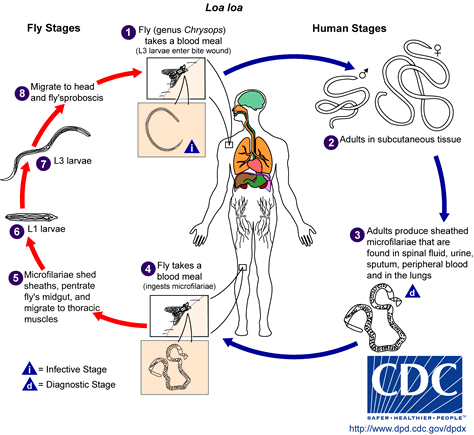
\includegraphics[width=0.7\textwidth]{figs/loa_loa_LifeCycle.png}
\end{center}

\end{frame}

\begin{frame}[fragile]{Data}

\begin{Shaded}
\begin{Highlighting}[]
\KeywordTok{library}\NormalTok{(PrevMap)}
\NormalTok{loaloa =}\StringTok{ }\KeywordTok{tbl_df}\NormalTok{(loaloa) }\OperatorTok\StringTok{ }\KeywordTok{setNames}\NormalTok{(., }\KeywordTok{tolower}\NormalTok{(}\KeywordTok{names}\NormalTok{(.)))}

\NormalTok{loaloa}
\NormalTok{## # A tibble: 197 × 11}
\NormalTok{##      row villcode longitude latitude no_exam no_inf elevation  mean9901 max9901}
\NormalTok{##    <int>    <int>     <dbl>    <dbl>   <int>  <int>     <int>     <dbl>   <dbl>}
\NormalTok{## 1      1      214  8.041860 5.736750     162      0       108 0.4389815    0.69}
\NormalTok{## 2      2      215  8.004330 5.680280     167      1        99 0.4258333    0.74}
\NormalTok{## 3      3      118  8.905556 5.347222      88      5       783 0.4914815    0.79}
\NormalTok{## 4      4      219  8.100720 5.917420      62      5       104 0.4324074    0.67}
\NormalTok{## 5      5      212  8.182510 5.104540     167      3       109 0.4150000    0.85}
\NormalTok{## 6      6      116  8.929167 5.355556      66      3       909 0.4363889    0.80}
\NormalTok{## 7      7       16 11.360000 4.885000     163     11       503 0.5019444    0.78}
\NormalTok{## 8      8      217  8.067490 5.897800      83      0       103 0.3731481    0.69}
\NormalTok{## 9      9      112  9.018056 5.593056      30      4       751 0.4808333    0.80}
\NormalTok{## 10    10      104  9.312500 6.004167      57      4       268 0.4865741    0.84}
\NormalTok{## # ... with 187 more rows, and 2 more variables: min9901 <dbl>, stdev9901 <dbl>}
\end{Highlighting}
\end{Shaded}

\end{frame}

\begin{frame}{Spatial Distribution}

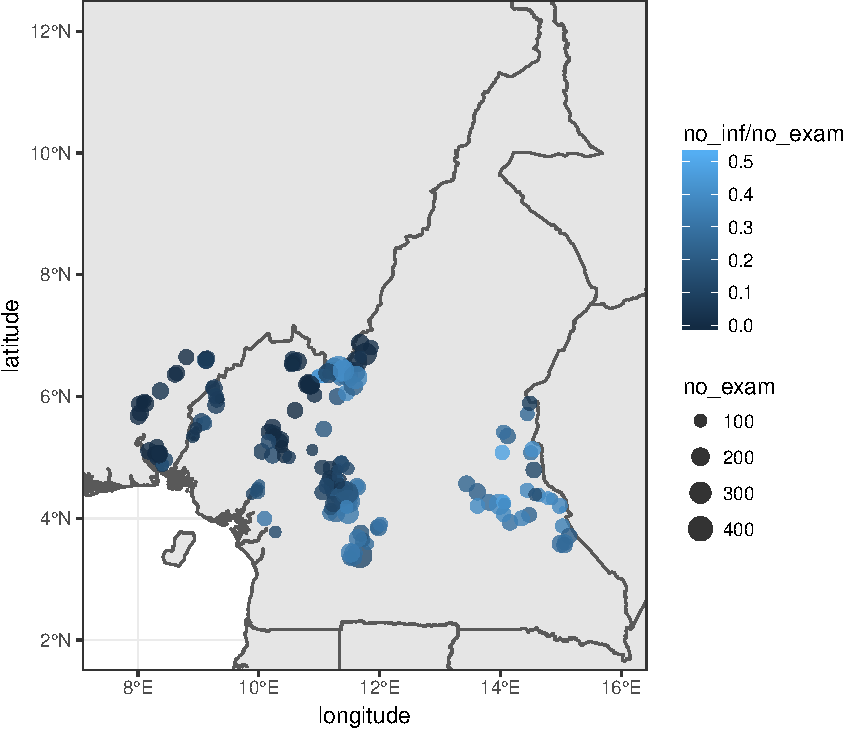
\includegraphics{Lec21_files/figure-beamer/unnamed-chunk-2-1.pdf}

\end{frame}

\begin{frame}[t]{Normalized Difference Vegetation Index (NVDI)}

\vspace{-2.5mm}

\begin{center}
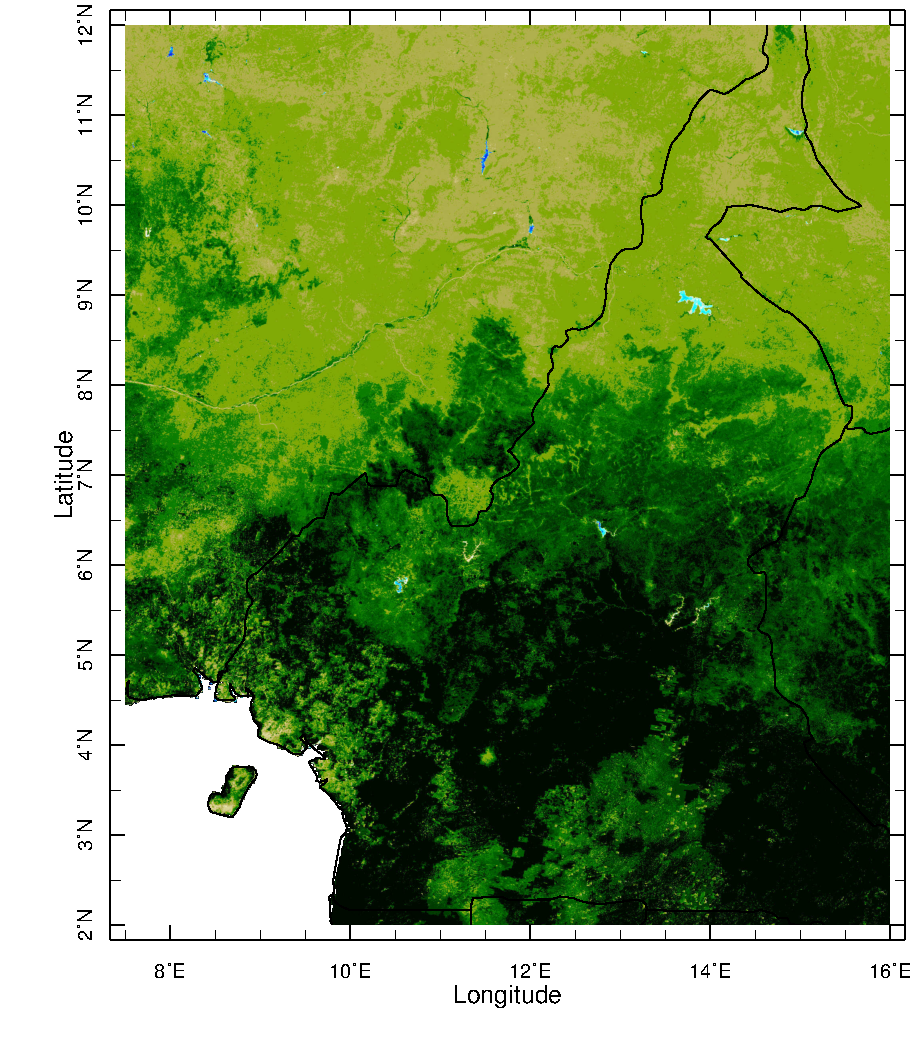
\includegraphics[width=0.6\textwidth]{figs/ndvi_cameroon.pdf} \\
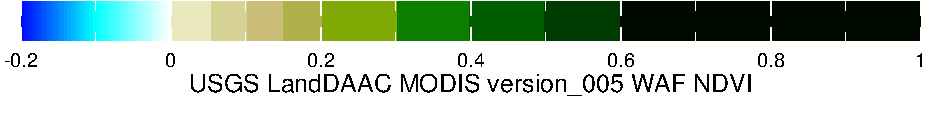
\includegraphics[width=0.6\textwidth]{figs/ndvi_cameroon_scale.pdf}
\end{center}

\end{frame}

\begin{frame}[fragile]{Paper / Data summary}

Original paper - Diggle, et. al. (2007). \emph{Spatial modelling and
prediction of Loa loa risk: decision making under uncertainty}. Annals
of Tropical Medicine and Parasitology, 101, 499-509.

\vspace{4mm}

\begin{itemize}
\tightlist
\item
  \texttt{no\_exam} and \texttt{no\_inf} - Collected between 1991 and
  2001 by NGOs (original paper mentions 168 villages and 21,938
  observations)
\end{itemize}

\vspace{2mm}

\begin{itemize}
\tightlist
\item
  \texttt{elevation} - USGS gtopo30 (1km resolution)
\end{itemize}

\vspace{2mm}

\begin{itemize}
\tightlist
\item
  \texttt{mean9901} to \texttt{stdev9901} - aggregated data from 1999 to
  2001 he Flemish Institute for Technological Research (1 km resolution)
\end{itemize}

\end{frame}

\begin{frame}{Diggle's Model}

\[ \log \left( \frac{p(x)}{1-p(x)} \right) = \alpha + f_1(\text{ELEVATION}) + f_2(\text{max (NDVI)}) + f_3(\text{sd (NDVI)}) + S(X) \]

where

\[ S(X) \sim \mathcal{N}(0, \Sigma) \]
\[ \{\Sigma\}_{ij} = \sigma^2 \, \exp(-d \,\phi) \]

\end{frame}

\begin{frame}{EDA}

\begin{center}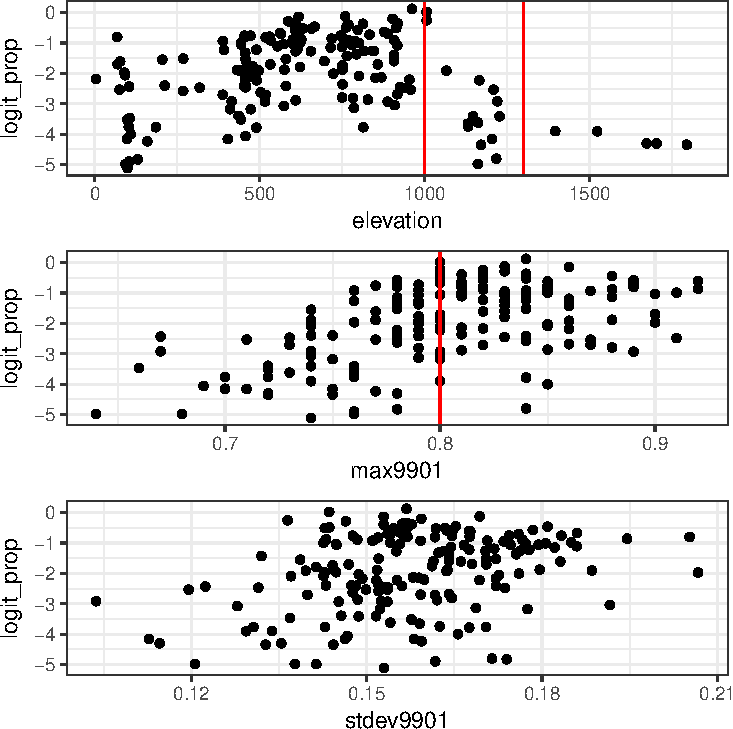
\includegraphics[width=0.8\textwidth]{Lec21_files/figure-beamer/unnamed-chunk-3-1} \end{center}

\end{frame}

\begin{frame}{Diggle's EDA}

\begin{center}
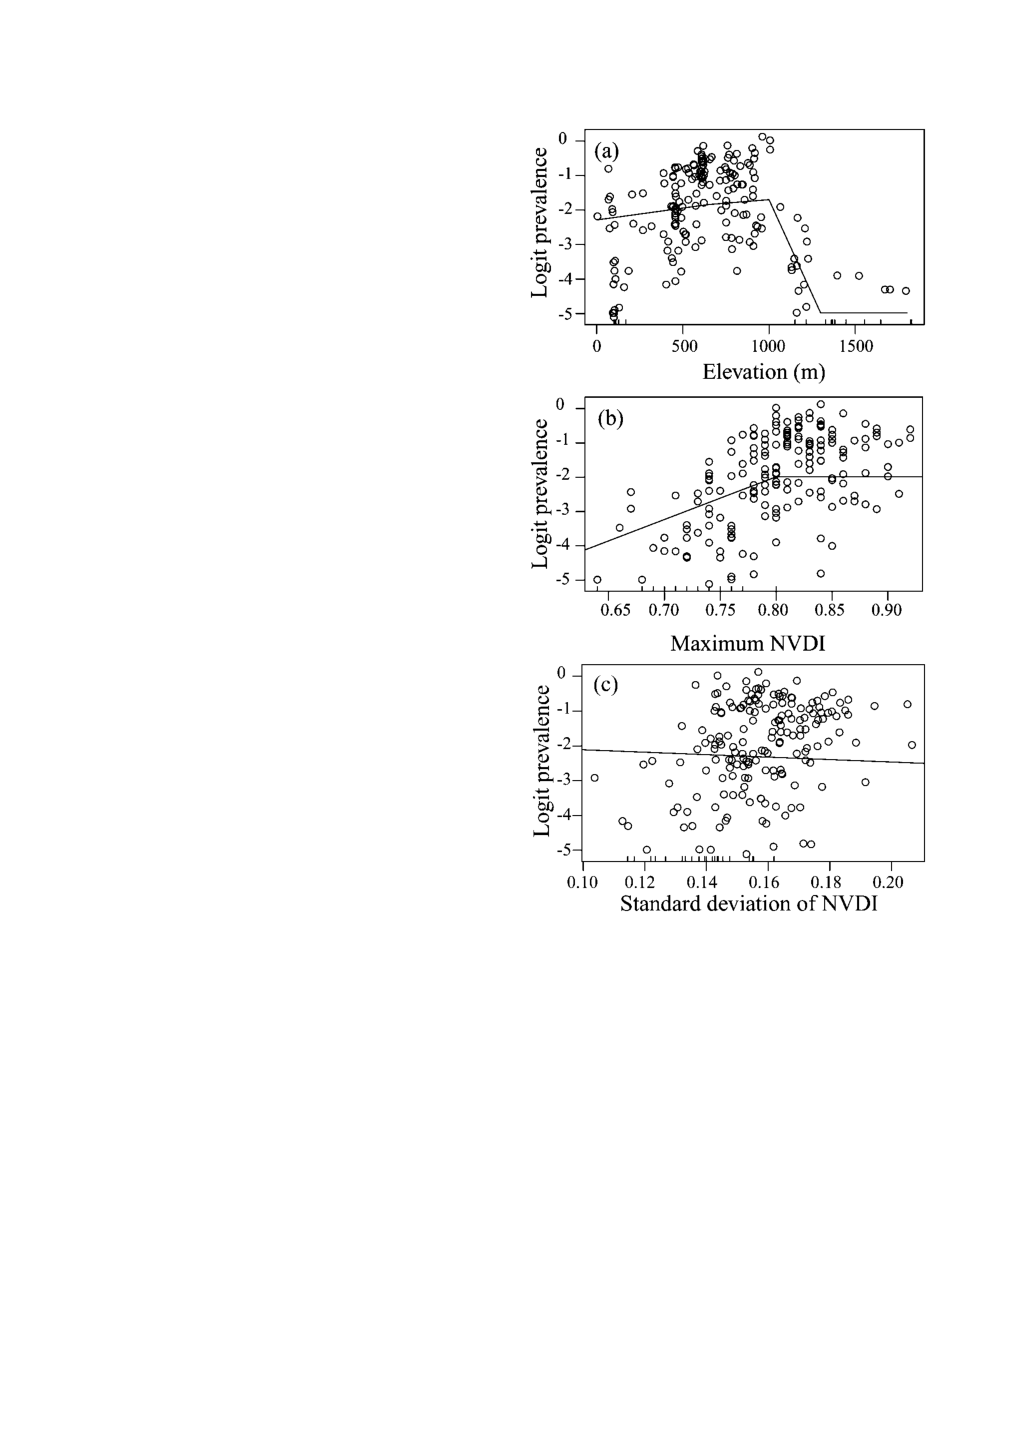
\includegraphics[width=0.7\textwidth]{figs/diggle_eda.pdf} \\
\end{center}

\end{frame}

\begin{frame}[fragile]{Model EDA}

\scriptoutput

\begin{Shaded}
\begin{Highlighting}[]
\NormalTok{loaloa =}\StringTok{ }\NormalTok{loaloa }\OperatorTok\StringTok{ }
\StringTok{  }\KeywordTok{mutate}\NormalTok{(}\DataTypeTok{elev_factor =} \KeywordTok{cut}\NormalTok{(elevation, }\DataTypeTok{breaks=}\KeywordTok{c}\NormalTok{(}\DecValTok{0}\NormalTok{,}\DecValTok{1000}\NormalTok{,}\DecValTok{1300}\NormalTok{,}\DecValTok{2000}\NormalTok{), }\DataTypeTok{dig.lab=}\DecValTok{5}\NormalTok{),}
         \DataTypeTok{max_factor  =} \KeywordTok{cut}\NormalTok{(max9901, }\DataTypeTok{breaks=}\KeywordTok{c}\NormalTok{(}\DecValTok{0}\NormalTok{,}\FloatTok{0.8}\NormalTok{,}\DecValTok{1}\NormalTok{)))}

\NormalTok{g =}\StringTok{ }\KeywordTok{glm}\NormalTok{(no_inf}\OperatorTok{/}\NormalTok{no_exam }\OperatorTok{~}\StringTok{ }\NormalTok{elevation}\OperatorTok{:}\NormalTok{elev_factor }\OperatorTok{+}\StringTok{ }\NormalTok{max9901}\OperatorTok{:}\NormalTok{max_factor }\OperatorTok{+}\StringTok{ }\NormalTok{stdev9901, }
        \DataTypeTok{data=}\NormalTok{loaloa, }\DataTypeTok{family=}\NormalTok{binomial, }\DataTypeTok{weights=}\NormalTok{loaloa}\OperatorTok{$}\NormalTok{no_exam)}

\KeywordTok{summary}\NormalTok{(g)}
\NormalTok{## }
\NormalTok{## Call:}
\NormalTok{## glm(formula = no_inf/no_exam ~ elevation:elev_factor + max9901:max_factor + }
\NormalTok{##     stdev9901, family = binomial, data = loaloa, weights = loaloa$no_exam)}
\NormalTok{## }
\NormalTok{## Deviance Residuals: }
\NormalTok{##     Min       1Q   Median       3Q      Max  }
\NormalTok{## -7.1434  -2.5887  -0.8993   1.6375  10.9052  }
\NormalTok{## }
\NormalTok{## Coefficients:}
\NormalTok{##                                    Estimate Std. Error z value Pr(>|z|)    }
\NormalTok{## (Intercept)                      -8.343e+00  4.825e-01 -17.291  < 2e-16 ***}
\NormalTok{## stdev9901                         8.781e+00  1.205e+00   7.288 3.14e-13 ***}
\NormalTok{## elevation:elev_factor(0,1000]     1.606e-03  8.749e-05  18.358  < 2e-16 ***}
\NormalTok{## elevation:elev_factor(1000,1300]  1.631e-04  8.792e-05   1.855   0.0636 .  }
\NormalTok{## elevation:elev_factor(1300,2000] -1.432e-03  1.887e-04  -7.588 3.25e-14 ***}
\NormalTok{## max9901:max_factor(0,0.8]         5.511e+00  6.299e-01   8.749  < 2e-16 ***}
\NormalTok{## max9901:max_factor(0.8,1]         5.626e+00  5.793e-01   9.711  < 2e-16 ***}
\NormalTok{## ---}
\NormalTok{## Signif. codes:  0 '***' 0.001 '**' 0.01 '*' 0.05 '.' 0.1 ' ' 1}
\NormalTok{## }
\NormalTok{## (Dispersion parameter for binomial family taken to be 1)}
\NormalTok{## }
\NormalTok{##     Null deviance: 4208.2  on 196  degrees of freedom}
\NormalTok{## Residual deviance: 2042.3  on 190  degrees of freedom}
\NormalTok{## AIC: 2804.6}
\NormalTok{## }
\NormalTok{## Number of Fisher Scoring iterations: 5}
\end{Highlighting}
\end{Shaded}

\end{frame}

\begin{frame}[fragile]{Residuals}

\scriptoutput

\begin{Shaded}
\begin{Highlighting}[]
\NormalTok{loaloa =}\StringTok{ }\NormalTok{loaloa }\OperatorTok\StringTok{ }
\StringTok{  }\KeywordTok{mutate}\NormalTok{(}\DataTypeTok{pred_prop =} \KeywordTok{predict}\NormalTok{(g, }\DataTypeTok{type=}\StringTok{"response"}\NormalTok{),}
         \DataTypeTok{resid =}\NormalTok{ prop }\OperatorTok{-}\StringTok{ }\NormalTok{pred_prop)}

\KeywordTok{ggplot}\NormalTok{(loaloa, }\KeywordTok{aes}\NormalTok{(}\DataTypeTok{x=}\NormalTok{prop, }\DataTypeTok{y=}\NormalTok{pred_prop)) }\OperatorTok{+}\StringTok{ }
\StringTok{  }\KeywordTok{geom_point}\NormalTok{() }\OperatorTok{+}
\StringTok{  }\KeywordTok{geom_abline}\NormalTok{(}\DataTypeTok{slope =} \DecValTok{1}\NormalTok{, }\DataTypeTok{intercept =} \DecValTok{0}\NormalTok{)}
\end{Highlighting}
\end{Shaded}

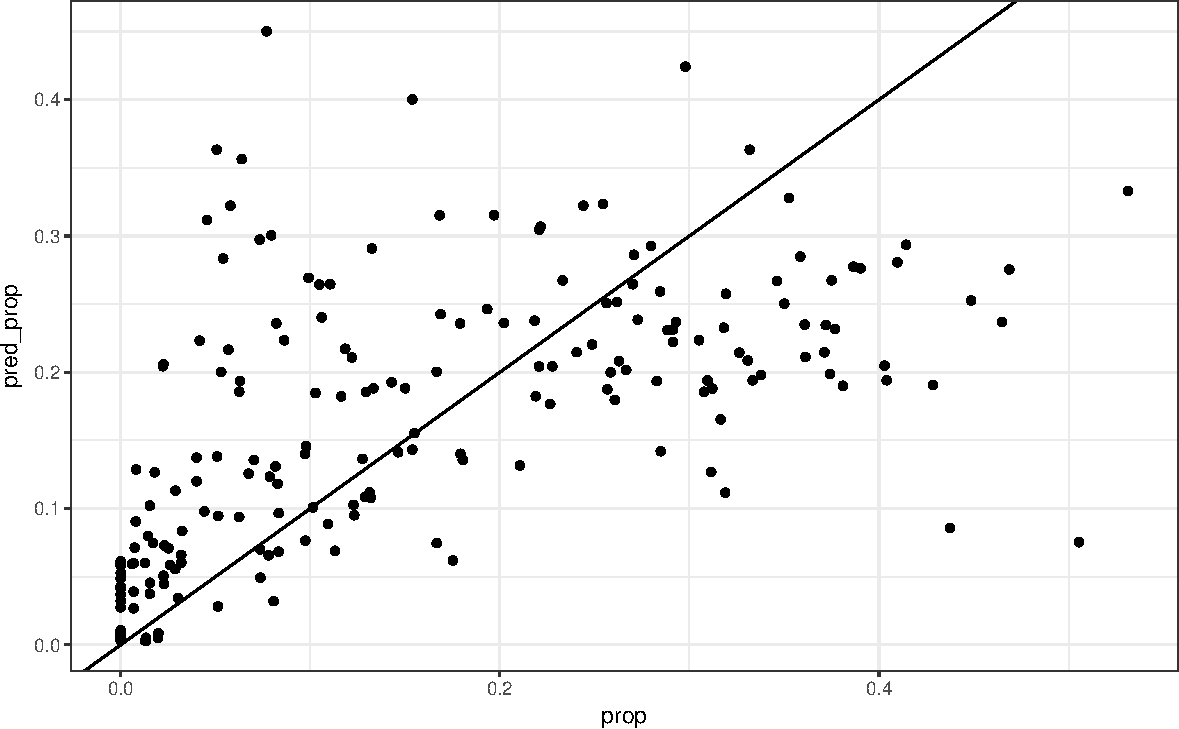
\includegraphics[width=0.75\textwidth]{Lec21_files/figure-beamer/unnamed-chunk-5-1}

\end{frame}

\begin{frame}[fragile]{Spatial Structure}

\begin{Shaded}
\begin{Highlighting}[]
\KeywordTok{library}\NormalTok{(geoR)}

\KeywordTok{variog}\NormalTok{(}\DataTypeTok{coords =} \KeywordTok{cbind}\NormalTok{(loaloa}\OperatorTok{$}\NormalTok{longitude, loaloa}\OperatorTok{$}\NormalTok{latitude), }
       \DataTypeTok{data =}\NormalTok{ loaloa}\OperatorTok{$}\NormalTok{resid,}
       \DataTypeTok{uvec =} \KeywordTok{seq}\NormalTok{(}\DecValTok{0}\NormalTok{, }\DecValTok{4}\NormalTok{, }\DataTypeTok{length.out =} \DecValTok{50}\NormalTok{)) }\OperatorTok\StringTok{ }\KeywordTok{plot}\NormalTok{()}
\NormalTok{## variog: computing omnidirectional variogram}
\end{Highlighting}
\end{Shaded}

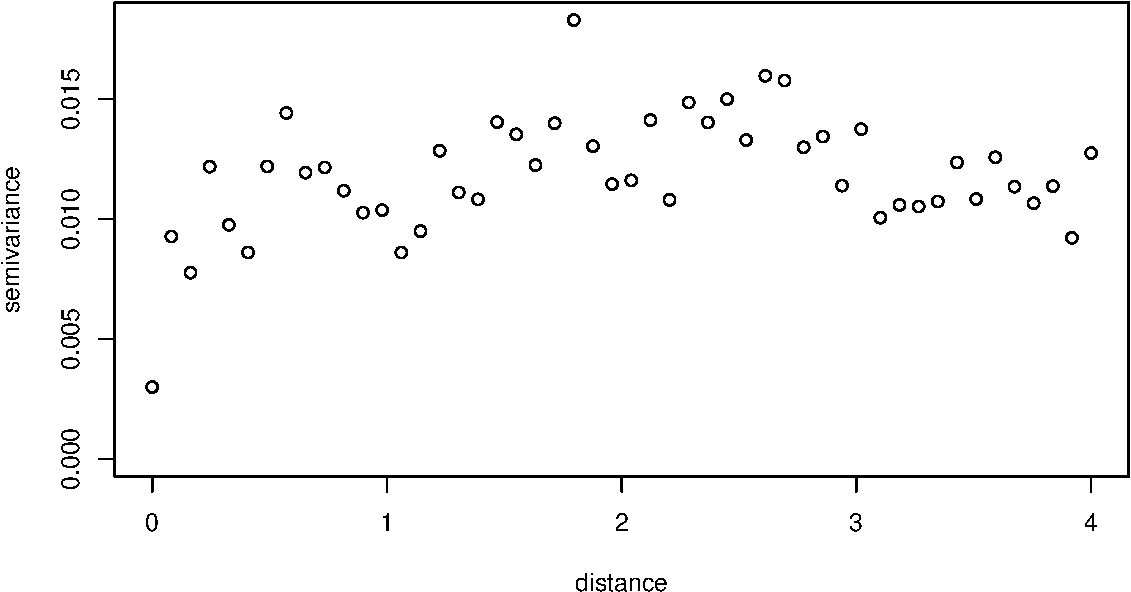
\includegraphics{Lec21_files/figure-beamer/unnamed-chunk-6-1.pdf}

\end{frame}

\begin{frame}[fragile,t]{\texttt{spBayes} GLM Model}

\scriptoutput

\begin{Shaded}
\begin{Highlighting}[]
\KeywordTok{library}\NormalTok{(spBayes)}

\NormalTok{spg =}\StringTok{ }\KeywordTok{spGLM}\NormalTok{(no_inf}\OperatorTok{/}\NormalTok{no_exam }\OperatorTok{~}\StringTok{ }\NormalTok{elevation}\OperatorTok{:}\NormalTok{elev_factor }\OperatorTok{+}\StringTok{ }\NormalTok{max9901}\OperatorTok{:}\NormalTok{max_factor }\OperatorTok{+}\StringTok{ }\NormalTok{stdev9901, }
            \DataTypeTok{data=}\NormalTok{loaloa, }\DataTypeTok{family=}\StringTok{"binomial"}\NormalTok{, }\DataTypeTok{weights=}\NormalTok{loaloa}\OperatorTok{$}\NormalTok{no_exam, }
            \DataTypeTok{coords=}\KeywordTok{cbind}\NormalTok{(loaloa}\OperatorTok{$}\NormalTok{longitude, loaloa}\OperatorTok{$}\NormalTok{latitude),}
            \DataTypeTok{cov.model=}\StringTok{"exponential"}\NormalTok{, }\DataTypeTok{n.samples=}\DecValTok{20000}\NormalTok{,}
            \CommentTok{#starting=list(beta=coefficients(g), phi=9, sigma.sq=1, w=0),}
            \DataTypeTok{starting=}\KeywordTok{list}\NormalTok{(}\DataTypeTok{beta=}\KeywordTok{rep}\NormalTok{(}\DecValTok{0}\NormalTok{,}\DecValTok{7}\NormalTok{), }\DataTypeTok{phi=}\DecValTok{3}\NormalTok{, }\DataTypeTok{sigma.sq=}\DecValTok{1}\NormalTok{, }\DataTypeTok{w=}\DecValTok{0}\NormalTok{),}
            \DataTypeTok{priors=}\KeywordTok{list}\NormalTok{(}\DataTypeTok{phi.unif=}\KeywordTok{c}\NormalTok{(}\FloatTok{0.1}\NormalTok{, }\DecValTok{10}\NormalTok{), }\DataTypeTok{sigma.sq.ig=}\KeywordTok{c}\NormalTok{(}\DecValTok{2}\NormalTok{, }\DecValTok{2}\NormalTok{)),}
            \DataTypeTok{amcmc=}\KeywordTok{list}\NormalTok{(}\DataTypeTok{n.batch=}\DecValTok{1000}\NormalTok{, }\DataTypeTok{batch.length=}\DecValTok{20}\NormalTok{, }\DataTypeTok{accept.rate=}\FloatTok{0.43}\NormalTok{))}

\KeywordTok{save}\NormalTok{(spg, loaloa, }\DataTypeTok{file=}\StringTok{"loaloa.Rdata"}\NormalTok{)}
\end{Highlighting}
\end{Shaded}

\end{frame}

\begin{frame}[fragile]{}

\footnotesize

\begin{Shaded}
\begin{Highlighting}[]
\NormalTok{spg}\OperatorTok{$}\NormalTok{p.beta.theta.samples }\OperatorTok\StringTok{ }
\StringTok{  }\KeywordTok{post_summary}\NormalTok{() }\OperatorTok\StringTok{ }
\StringTok{  }\NormalTok{knitr}\OperatorTok{::}\KeywordTok{kable}\NormalTok{(}\DataTypeTok{digits=}\DecValTok{5}\NormalTok{)}
\end{Highlighting}
\end{Shaded}

\begin{longtable}[]{@{}lrrrr@{}}
\toprule
param & post\_mean & post\_med & post\_lower &
post\_upper\tabularnewline
\midrule
\endhead
(Intercept) & -12.69885 & -11.61326 & -21.65388 &
-6.96361\tabularnewline
stdev9901 & 9.24231 & 9.15244 & -14.48649 & 29.76058\tabularnewline
elevation:elev\_factor(0,1000{]} & 0.00048 & 0.00077 & -0.00474 &
0.00291\tabularnewline
elevation:elev\_factor(1000,1300{]} & -0.00048 & -0.00032 & -0.00359 &
0.00169\tabularnewline
elevation:elev\_factor(1300,2000{]} & -0.00814 & -0.00581 & -0.02900 &
0.00004\tabularnewline
max9901:max\_factor(0,0.8{]} & 4.87762 & 3.99492 & -2.93030 &
15.63246\tabularnewline
max9901:max\_factor(0.8,1{]} & 5.08690 & 4.44632 & -2.18626 &
14.89011\tabularnewline
sigma.sq & 0.38088 & 0.34626 & 0.12793 & 0.88673\tabularnewline
phi & 6.22996 & 5.18205 & 0.69584 & 18.67107\tabularnewline
\bottomrule
\end{longtable}

\end{frame}

\begin{frame}{Prediction}

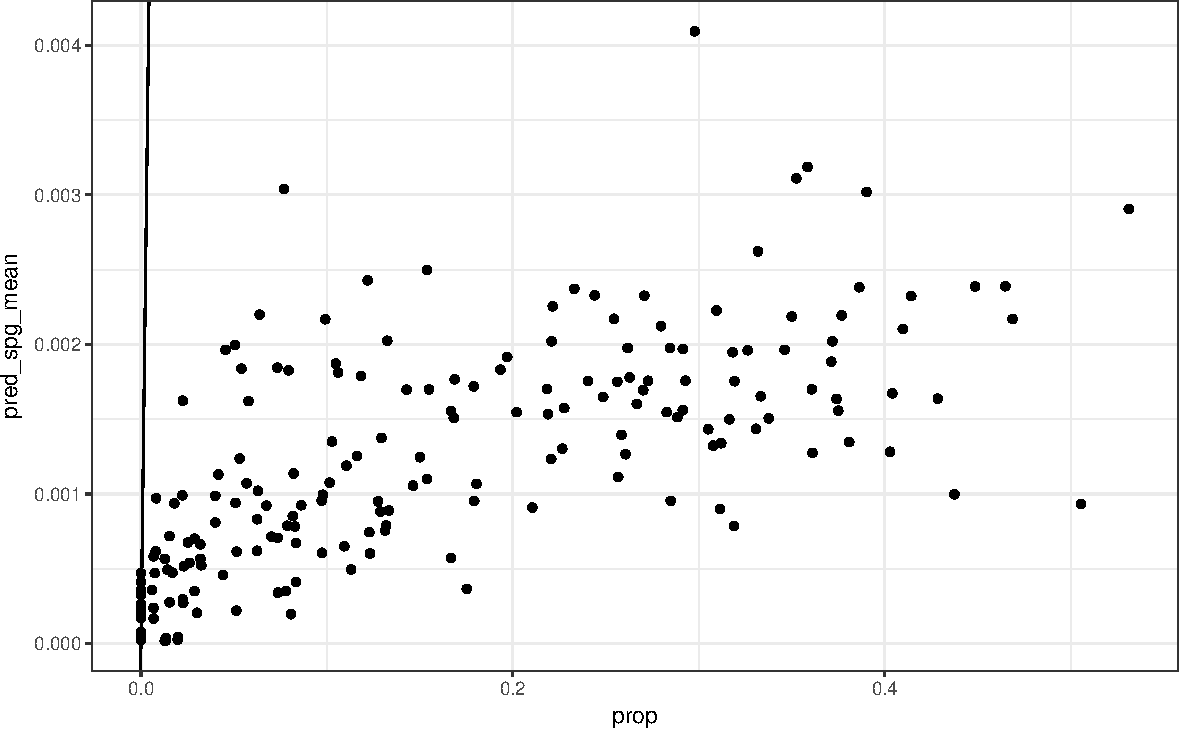
\includegraphics{Lec21_files/figure-beamer/unnamed-chunk-10-1.pdf}

\end{frame}

\begin{frame}[fragile,t]{\texttt{spBayes} GLM Model - Fixed?}

\scriptoutput

\begin{Shaded}
\begin{Highlighting}[]
\KeywordTok{library}\NormalTok{(spBayes)}

\NormalTok{spg_good =}\StringTok{ }\KeywordTok{spGLM}\NormalTok{(no_inf }\OperatorTok{~}\StringTok{ }\NormalTok{elevation}\OperatorTok{:}\NormalTok{elev_factor }\OperatorTok{+}\StringTok{ }\NormalTok{max9901}\OperatorTok{:}\NormalTok{max_factor }\OperatorTok{+}\StringTok{ }\NormalTok{stdev9901, }
                 \DataTypeTok{data=}\NormalTok{loaloa, }\DataTypeTok{family=}\StringTok{"binomial"}\NormalTok{, }\DataTypeTok{weights=}\NormalTok{loaloa}\OperatorTok{$}\NormalTok{no_exam, }
                 \DataTypeTok{coords=}\KeywordTok{cbind}\NormalTok{(loaloa}\OperatorTok{$}\NormalTok{longitude, loaloa}\OperatorTok{$}\NormalTok{latitude),}
                 \DataTypeTok{cov.model=}\StringTok{"exponential"}\NormalTok{, }\DataTypeTok{n.samples=}\DecValTok{20000}\NormalTok{,}
                 \CommentTok{#starting=list(beta=coefficients(g), phi=9, sigma.sq=1, w=0),}
                 \DataTypeTok{starting=}\KeywordTok{list}\NormalTok{(}\DataTypeTok{beta=}\KeywordTok{rep}\NormalTok{(}\DecValTok{0}\NormalTok{,}\DecValTok{7}\NormalTok{), }\DataTypeTok{phi=}\DecValTok{3}\NormalTok{, }\DataTypeTok{sigma.sq=}\DecValTok{1}\NormalTok{, }\DataTypeTok{w=}\DecValTok{0}\NormalTok{),}
                 \DataTypeTok{priors=}\KeywordTok{list}\NormalTok{(}\DataTypeTok{phi.unif=}\KeywordTok{c}\NormalTok{(}\FloatTok{0.1}\NormalTok{, }\DecValTok{10}\NormalTok{), }\DataTypeTok{sigma.sq.ig=}\KeywordTok{c}\NormalTok{(}\DecValTok{2}\NormalTok{, }\DecValTok{2}\NormalTok{)),}
                 \DataTypeTok{amcmc=}\KeywordTok{list}\NormalTok{(}\DataTypeTok{n.batch=}\DecValTok{1000}\NormalTok{, }\DataTypeTok{batch.length=}\DecValTok{20}\NormalTok{, }\DataTypeTok{accept.rate=}\FloatTok{0.43}\NormalTok{))}

\KeywordTok{save}\NormalTok{(spg_good, loaloa, }\DataTypeTok{file=}\StringTok{"loaloa_good.Rdata"}\NormalTok{)}
\end{Highlighting}
\end{Shaded}

\end{frame}

\begin{frame}[fragile]{}

\footnotesize

\begin{Shaded}
\begin{Highlighting}[]
\NormalTok{spg_good}\OperatorTok{$}\NormalTok{p.beta.theta.samples }\OperatorTok\StringTok{ }
\StringTok{  }\KeywordTok{post_summary}\NormalTok{() }\OperatorTok\StringTok{ }
\StringTok{  }\NormalTok{knitr}\OperatorTok{::}\KeywordTok{kable}\NormalTok{(}\DataTypeTok{digits=}\DecValTok{5}\NormalTok{)}
\end{Highlighting}
\end{Shaded}

\begin{longtable}[]{@{}lrrrr@{}}
\toprule
param & post\_mean & post\_med & post\_lower &
post\_upper\tabularnewline
\midrule
\endhead
(Intercept) & -2.66090 & -2.13138 & -6.31576 & -0.80487\tabularnewline
stdev9901 & -0.12840 & -0.41947 & -5.86766 & 8.58835\tabularnewline
elevation:elev\_factor(0,1000{]} & 0.00023 & 0.00024 & -0.00051 &
0.00086\tabularnewline
elevation:elev\_factor(1000,1300{]} & -0.00054 & -0.00055 & -0.00128 &
0.00020\tabularnewline
elevation:elev\_factor(1300,2000{]} & -0.00204 & -0.00200 & -0.00285 &
-0.00127\tabularnewline
max9901:max\_factor(0,0.8{]} & 0.88041 & 0.90550 & -1.03795 &
3.63477\tabularnewline
max9901:max\_factor(0.8,1{]} & 1.28673 & 1.13796 & -0.26884 &
3.83860\tabularnewline
sigma.sq & 1.47552 & 1.39146 & 0.43359 & 3.05883\tabularnewline
phi & 2.22372 & 2.09524 & 0.86456 & 4.14663\tabularnewline
\bottomrule
\end{longtable}

\end{frame}

\begin{frame}{Prediction}

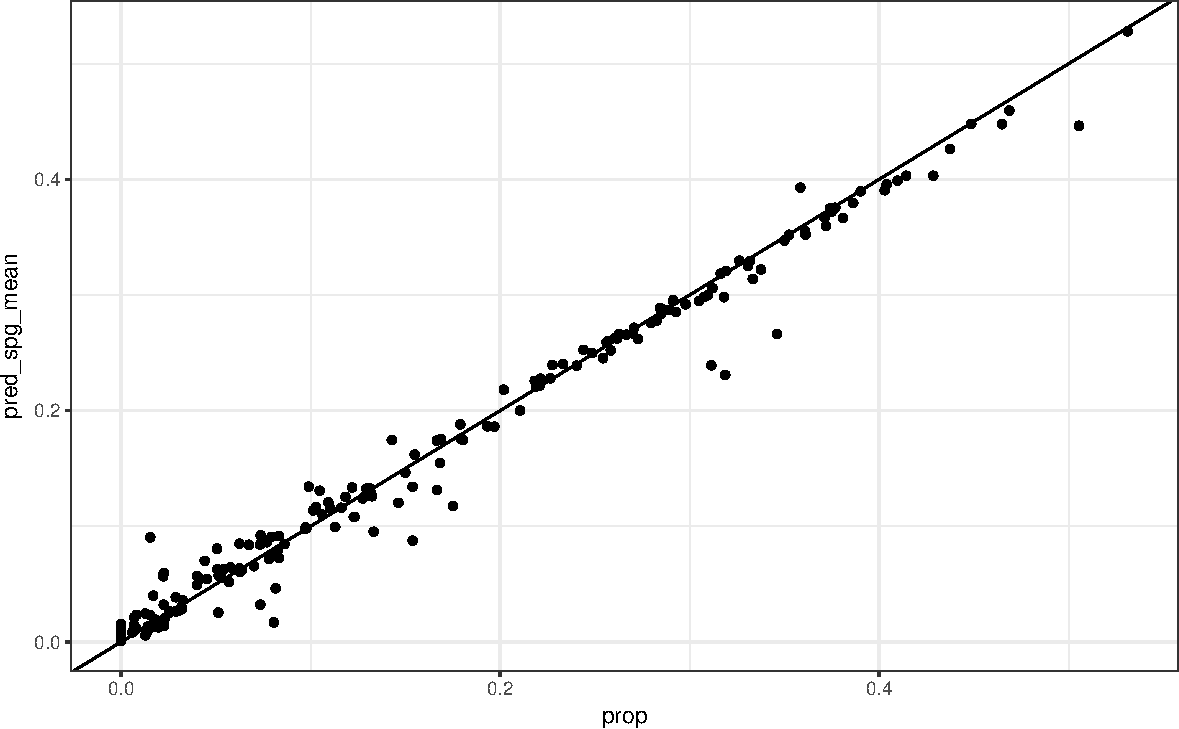
\includegraphics{Lec21_files/figure-beamer/unnamed-chunk-14-1.pdf}

\end{frame}

\begin{frame}{Diggle's Predictive Surface}

\begin{center}
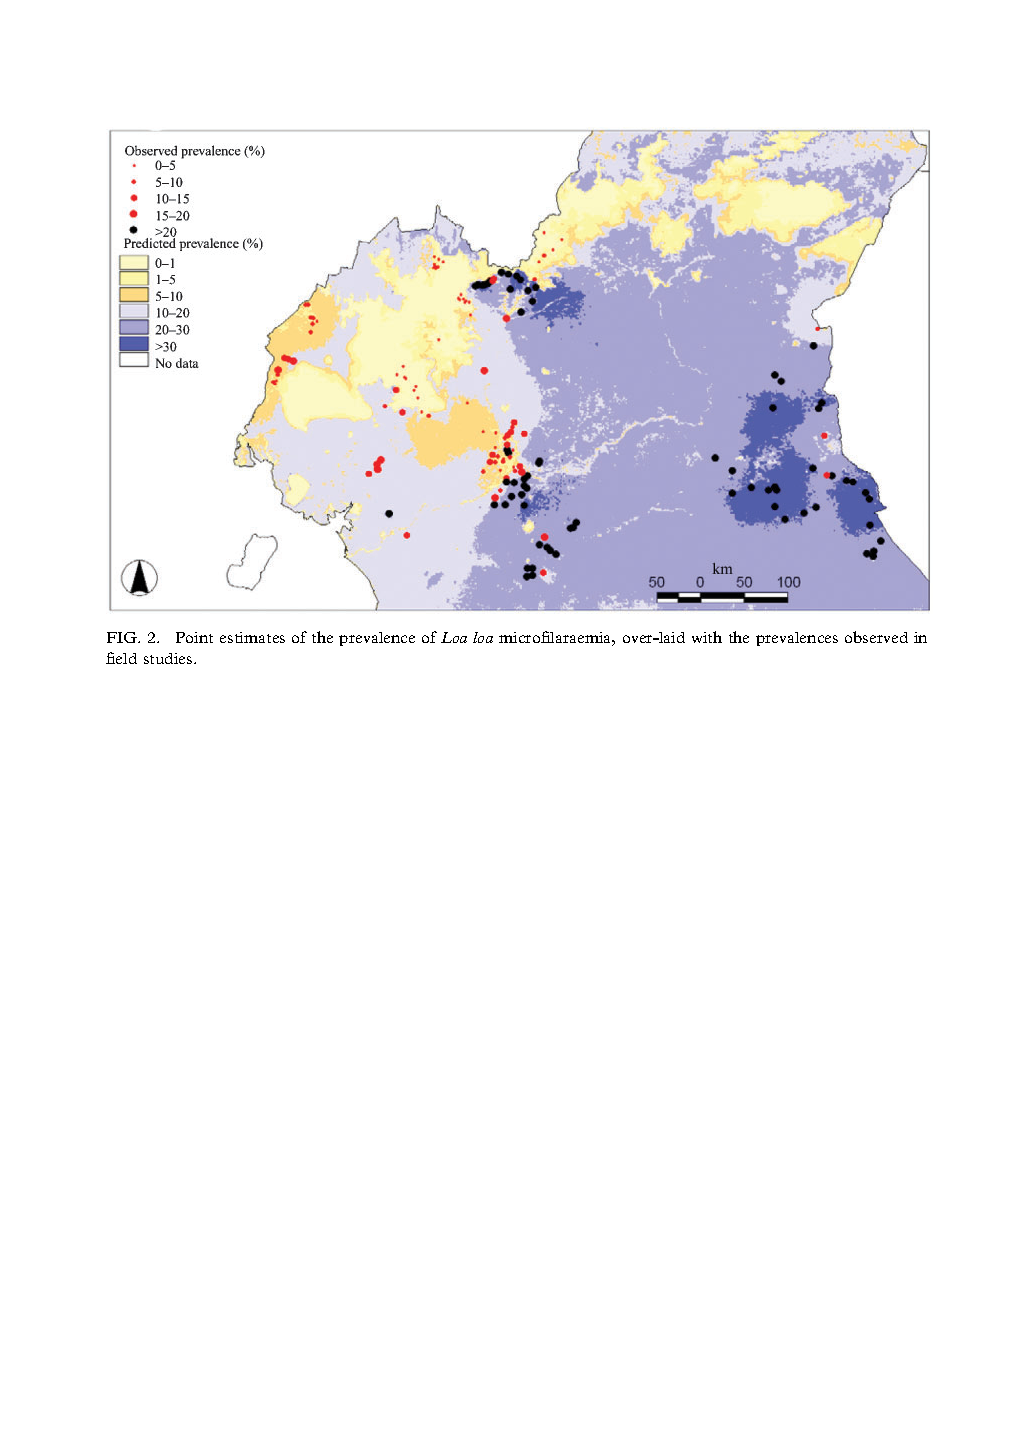
\includegraphics[width=0.9\textwidth]{figs/diggle_fig2.pdf}
\end{center}

\end{frame}

\begin{frame}{Exceedance Probability - Posterior Summary}

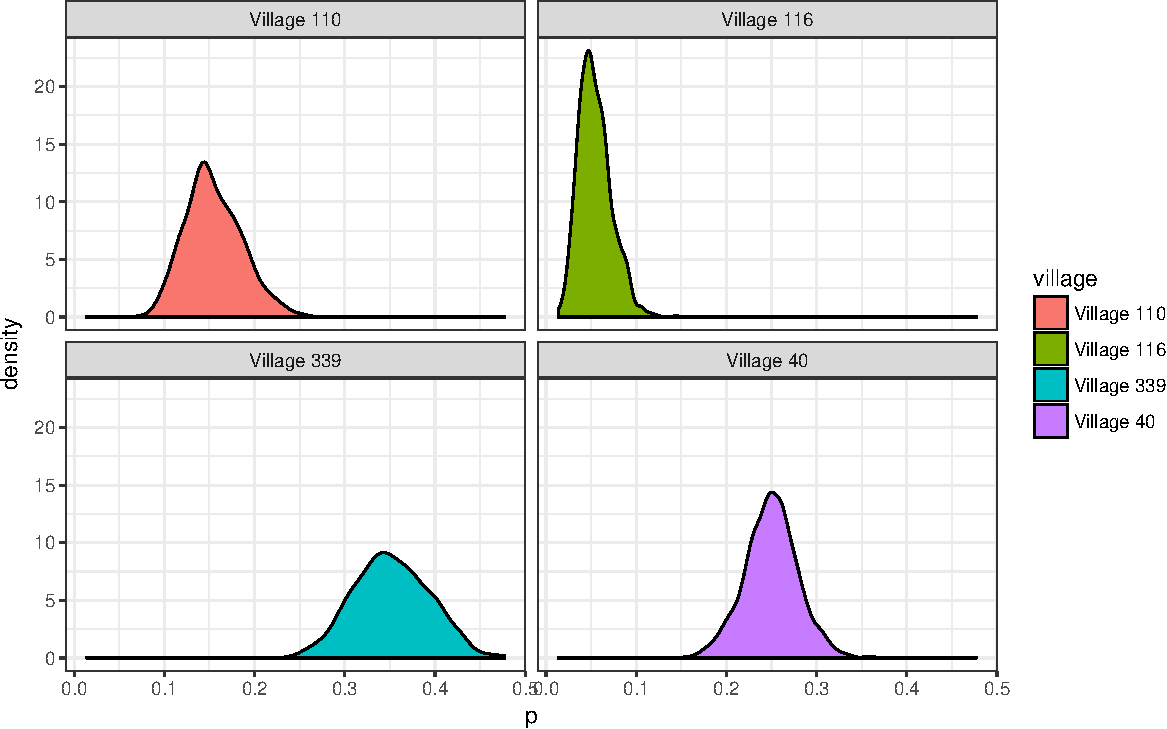
\includegraphics{Lec21_files/figure-beamer/unnamed-chunk-15-1.pdf}

\end{frame}

\begin{frame}{Exceedance Probability Predictive Surface}

\begin{center}
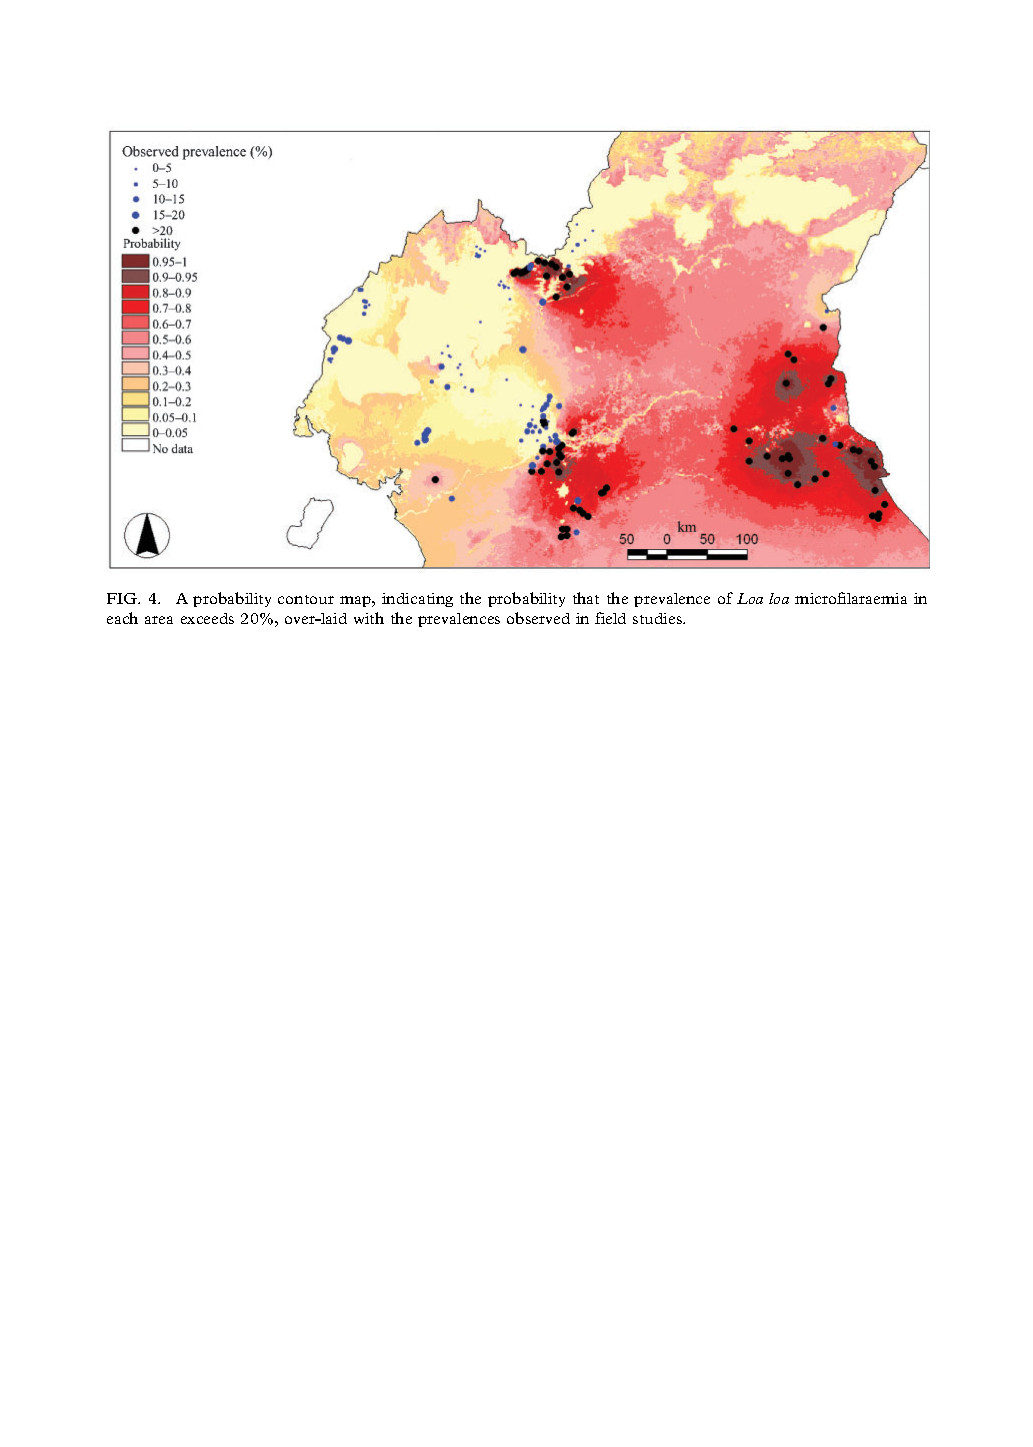
\includegraphics[width=0.9\textwidth]{figs/diggle_fig4.pdf}
\end{center}

\end{frame}

\section{Spatial Assignment of Migratory
Birds}\label{spatial-assignment-of-migratory-birds}

\begin{frame}{Background}

Using intrinsic markers (genetic and isotopic signals) for the purpose
of inferring migratory connectivity.

\vspace{2mm}

\begin{itemize}
\tightlist
\item
  Existing methods are too coarse for most applications
\end{itemize}

\vspace{2mm}

\begin{itemize}
\tightlist
\item
  Large amounts of data are available ( \textgreater{}150,000 feather
  samples from \textgreater{}500 species)
\end{itemize}

\vspace{2mm}

\begin{itemize}
\tightlist
\item
  Genetic assignment methods are based on Wasser, et al. (2004)
\end{itemize}

\vspace{2mm}

\begin{itemize}
\tightlist
\item
  Isotopic assignment methods are based on Wunder, et al. (2005)
\end{itemize}

\end{frame}

\begin{frame}{Data - DNA microsatellites and \(\delta \isotope[2]{H}\)}

\begin{columns}[t]
\column{0.5\textwidth}
Hermit Thrush (\textit{Catharus guttatus}) \\
\vspace{2mm}
\begin{itemize}
\item 138 individuals
\item 14 locations
\item 6 loci
\item 9-27 alleles / locus
\end{itemize}
\column{0.5\textwidth}
Wilson's Warbler (\textit{Wilsonia pusilla}) \\
\vspace{2mm}
\begin{itemize}
\item 163 individuals
\item 8 locations
\item 9 loci
\item 15-31 alleles / locus
\end{itemize}

\end{columns}

\vspace{5mm}

\begin{columns}[t]
\column{0.5\textwidth}
\begin{center}
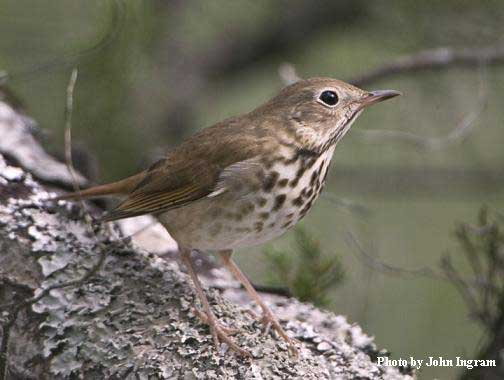
\includegraphics[width=0.65\textwidth]{figs/hermit_thrush.jpeg}
\end{center}
\column{0.5\textwidth}
\begin{center}
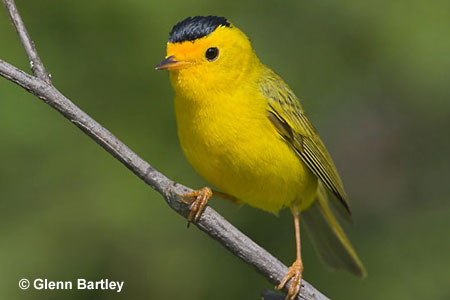
\includegraphics[width=0.65\textwidth]{figs/wilsons_warbler.jpeg}
\end{center}
\end{columns}

\end{frame}

\begin{frame}{Sampling Locations}

\begin{center}
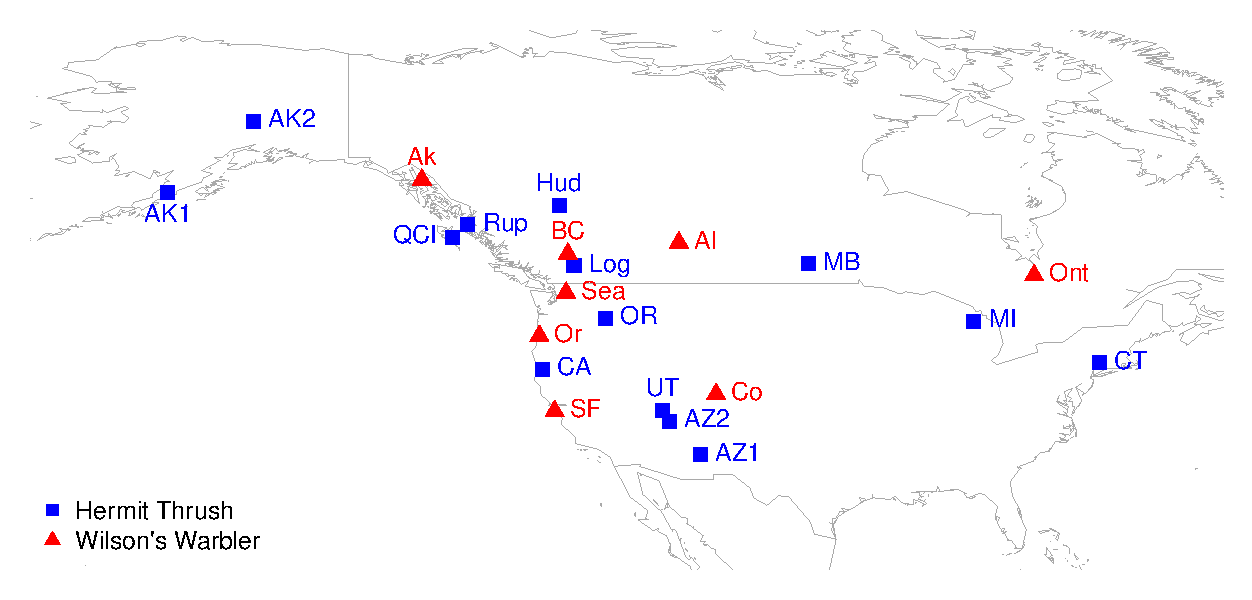
\includegraphics[width=\textwidth]{figs/sampling_locs.pdf}
\end{center}

\end{frame}

\begin{frame}{Allele Frequency Model}

For the allele \(i\), from locus \(l\), at location \(k\)

\[
\begin{aligned}
\bm{y}_{\cdot l k}|\bm{\Theta} &\sim \mathcal{N}\left(\textstyle\sum_i y_{ilk},\: \bm{f}_{\cdot l k}\right) \\
\\
f_{ilk} &= \frac{\exp(\Theta_{ilk})}{\sum_i \exp(\Theta_{ilk})} \\
\\
\bm{\Theta}_{il}|\bm{\alpha},\bm{\mu} &\sim \mathcal{N}( \bm{\mu}_{il},\, \bm{\Sigma_{}}) \\
\end{aligned}
\]

\[ \left\{\Sigma\right\}_{ij} = \sigma^2 \, \exp \Big(-(\{d\}_{ij}\, r)^{\psi} \Big) + \sigma^2_n \, {1}_{i=j} \]

\end{frame}

\begin{frame}{Predictions by Allele (Locus 3)}

\begin{center}
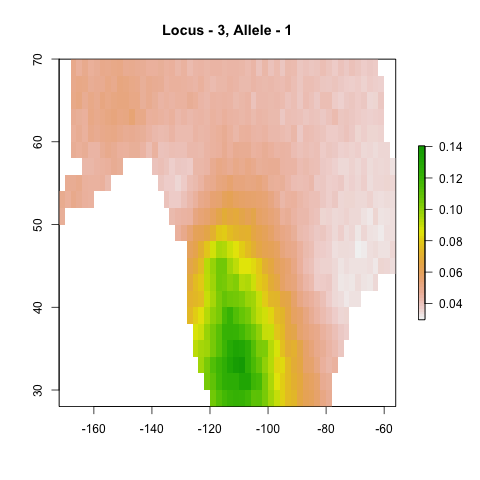
\includegraphics[width=0.25\textwidth]{figs/allele3/Med-Al3-1.png}
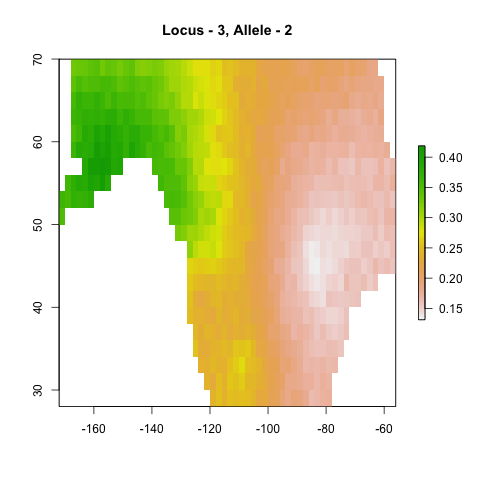
\includegraphics[width=0.25\textwidth]{figs/allele3/Med-Al3-2.png}
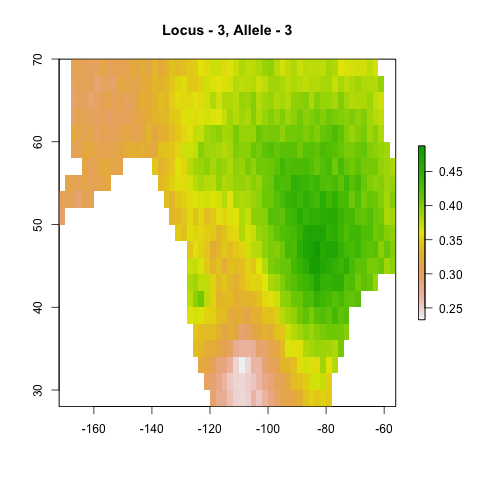
\includegraphics[width=0.25\textwidth]{figs/allele3/Med-Al3-3.png} \\
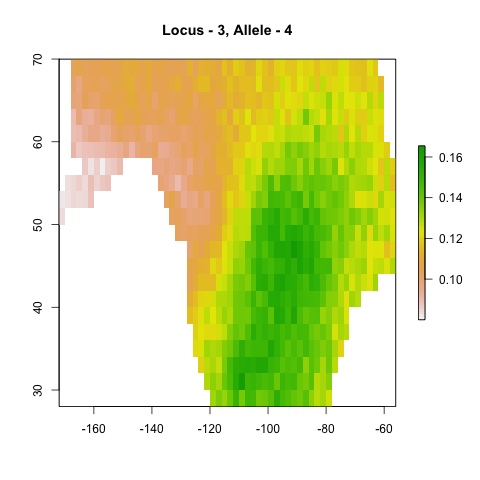
\includegraphics[width=0.25\textwidth]{figs/allele3/Med-Al3-4.png}
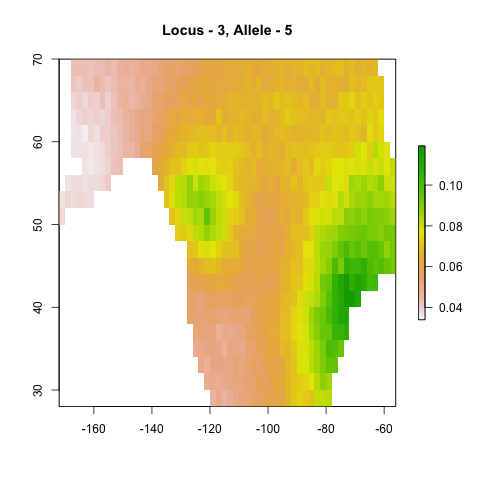
\includegraphics[width=0.25\textwidth]{figs/allele3/Med-Al3-5.png}
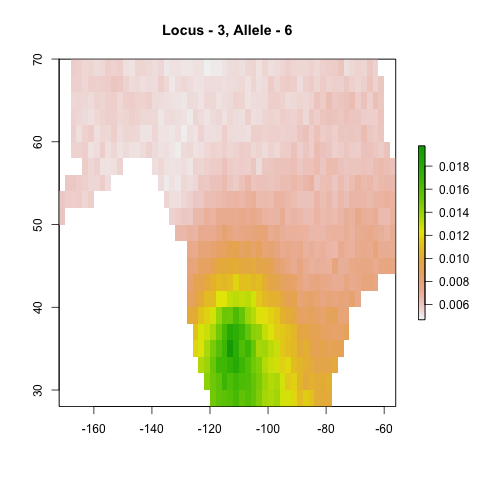
\includegraphics[width=0.25\textwidth]{figs/allele3/Med-Al3-6.png} \\
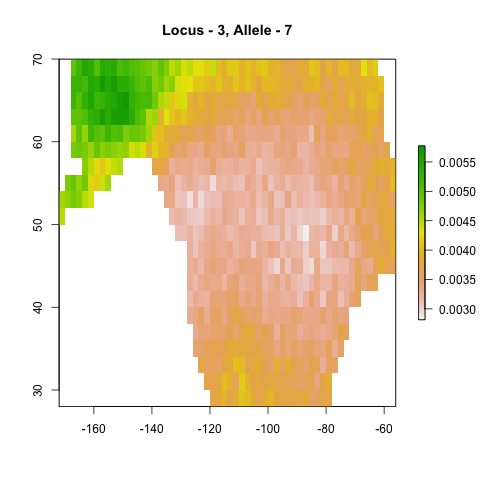
\includegraphics[width=0.25\textwidth]{figs/allele3/Med-Al3-7.png}
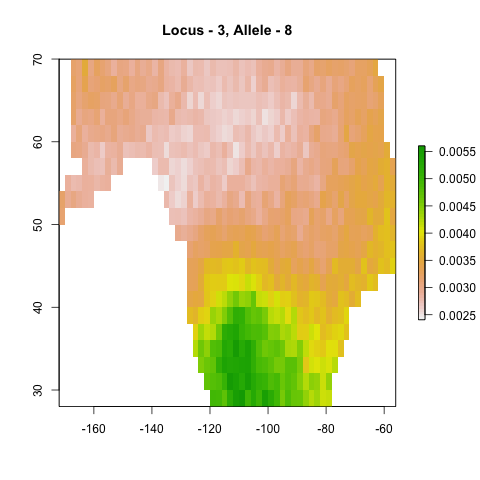
\includegraphics[width=0.25\textwidth]{figs/allele3/Med-Al3-8.png}
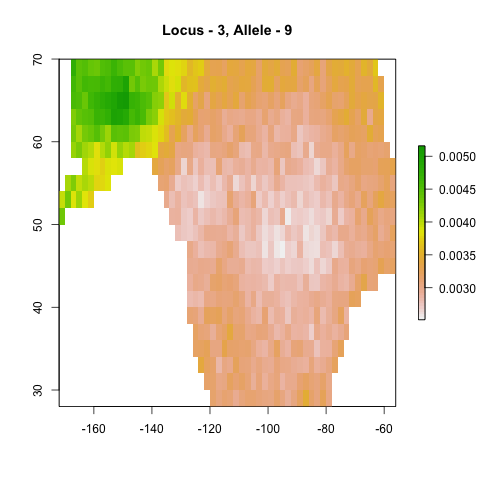
\includegraphics[width=0.25\textwidth]{figs/allele3/Med-Al3-9.png}
\end{center}

\end{frame}

\begin{frame}{Genetic Assignment Model}

Assignment model assuming Hardy-Weinberg equilibrium and allowing for
genotyping (\(\delta\)) and single amplification (\(\gamma\)) errors.

\[
\begin{aligned}
P(S_G|\bm{f},k) &= \prod_l P(i_l, j_l | \bm{f},k) \\
\\
P(i_l, j_l | \bm{f},k) &= 
\begin{cases}
\gamma P(i_l|\bm{f},k) + (1-\gamma)P(i_l|\bm{\tilde f},k)^2 & \text{if $i=j$} \vspace{2mm} \\
(1-\gamma) P(i_l|\bm{f},k) P(j_l|\bm{f},k)      & \text{if $i \ne j$}
\end{cases} \\
\\
P(i_l|\bm{f},k) &= (1-\delta) f_{lik} + \delta / m_l
\end{aligned}
\]

\end{frame}

\begin{frame}{Combined Model}

\begin{center}
Genetic \qquad\qquad\qquad\quad
Isotopic \qquad\qquad\qquad\quad
Combined
\end{center}

\begin{center}
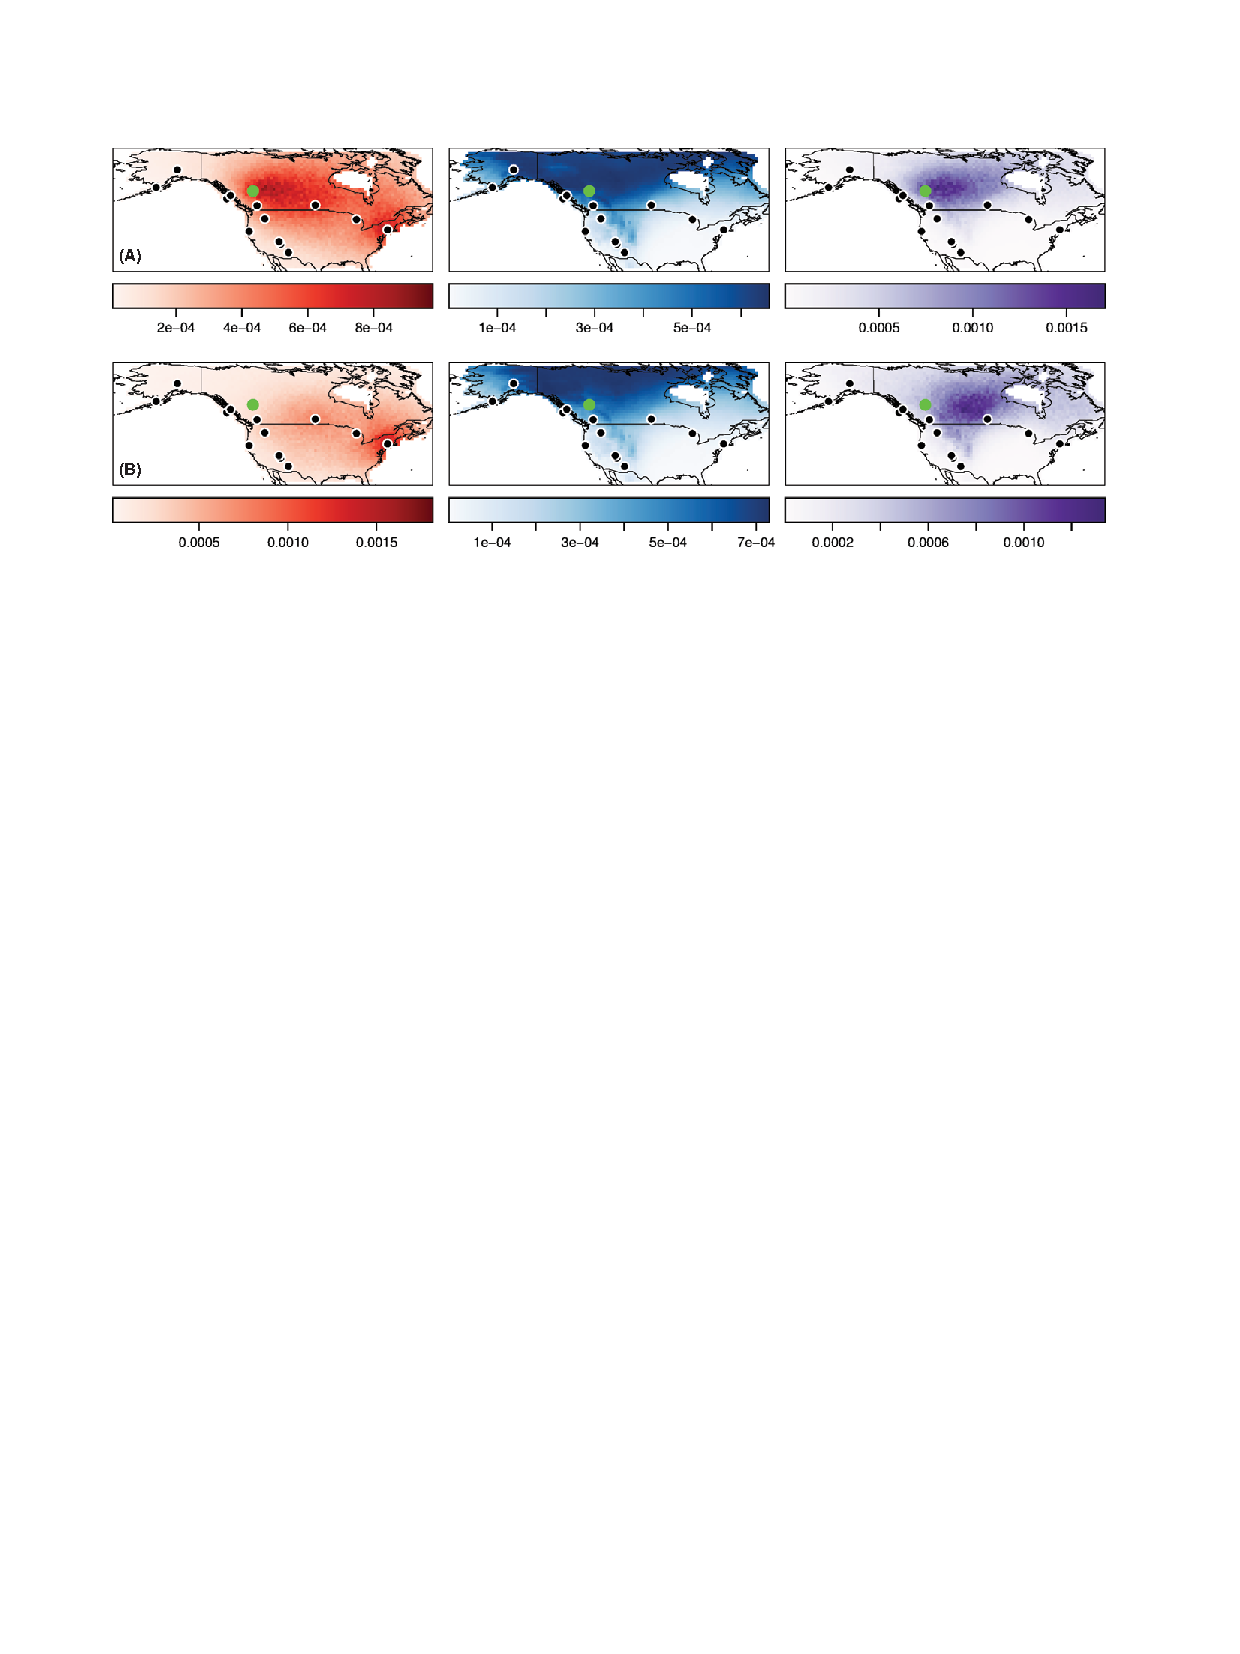
\includegraphics[width=\textwidth]{figs/hermit_maps.pdf}
\end{center}

\end{frame}

\begin{frame}{Model Assessment}

\begin{center}
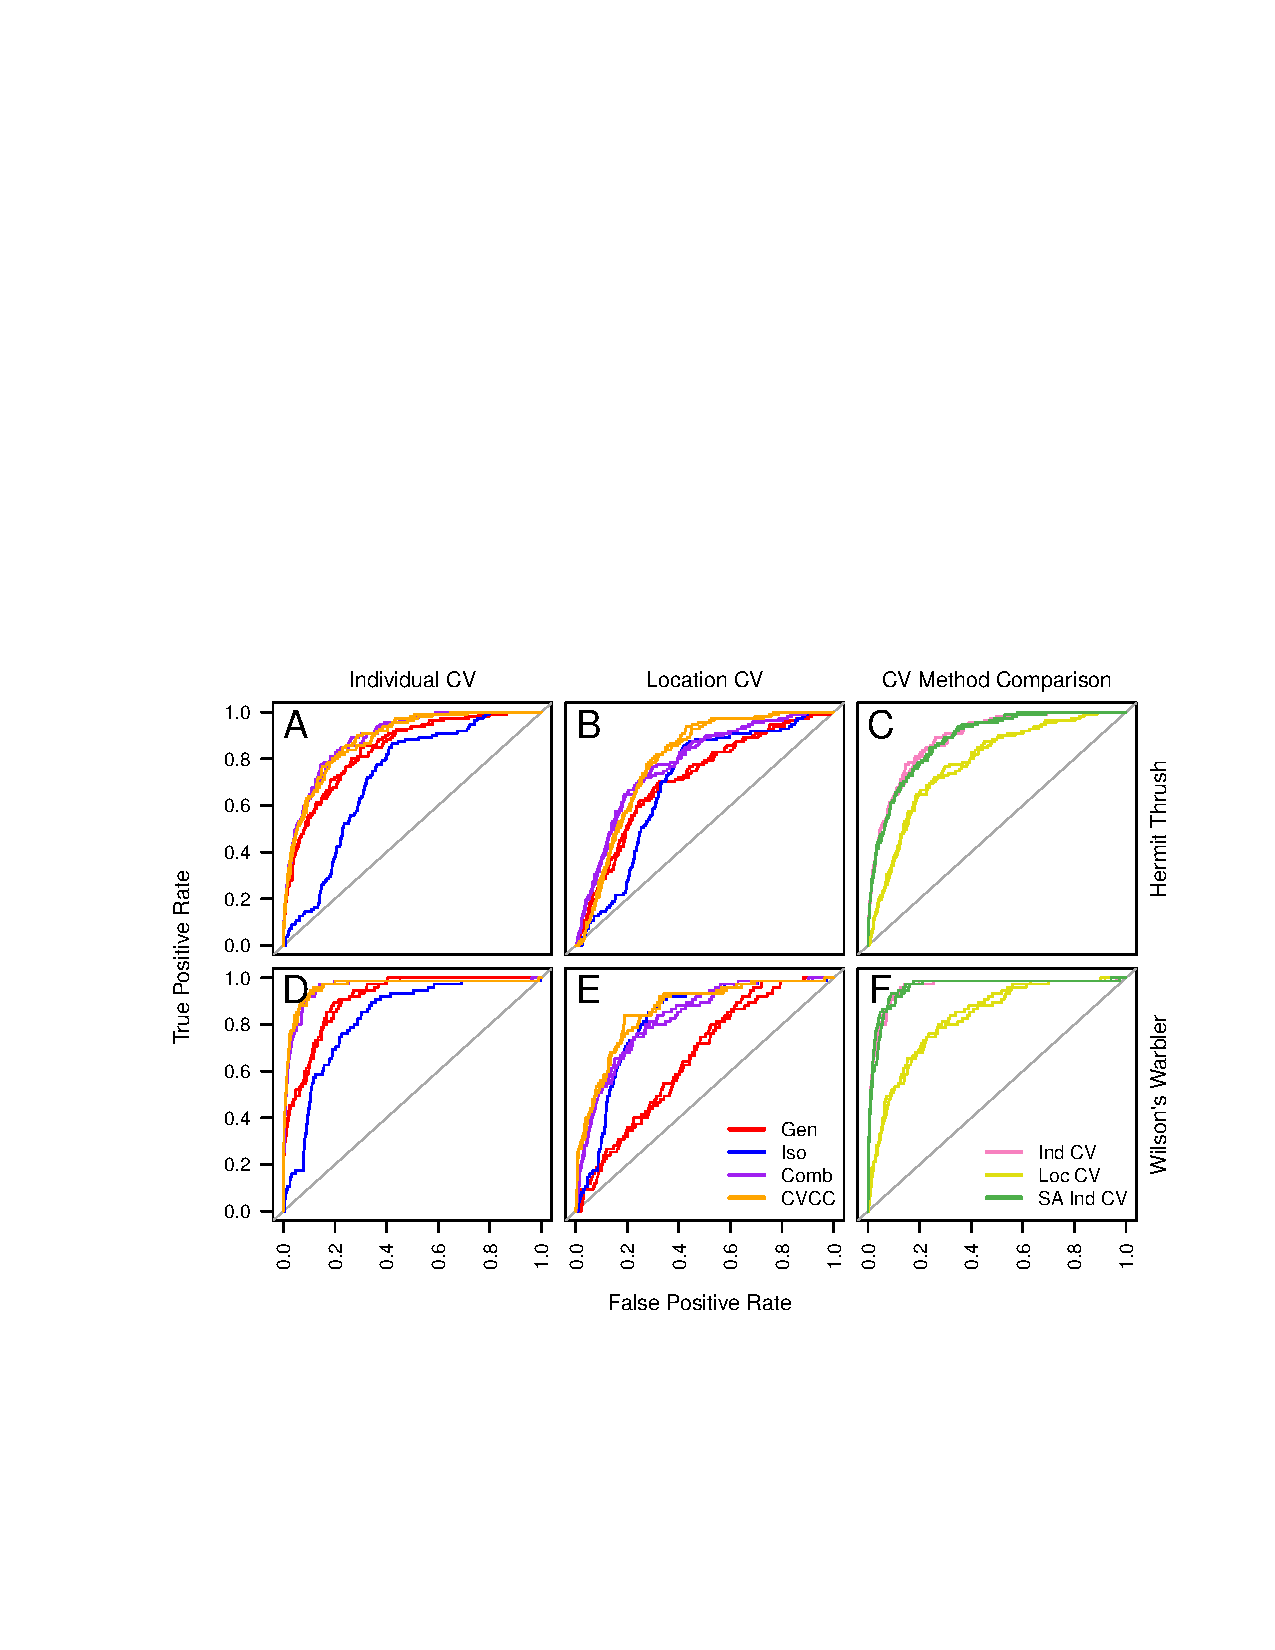
\includegraphics[width=\textwidth]{figs/ROCs.pdf}
\end{center}

\end{frame}

\begin{frame}{Migratory Connectivity}

\begin{center}
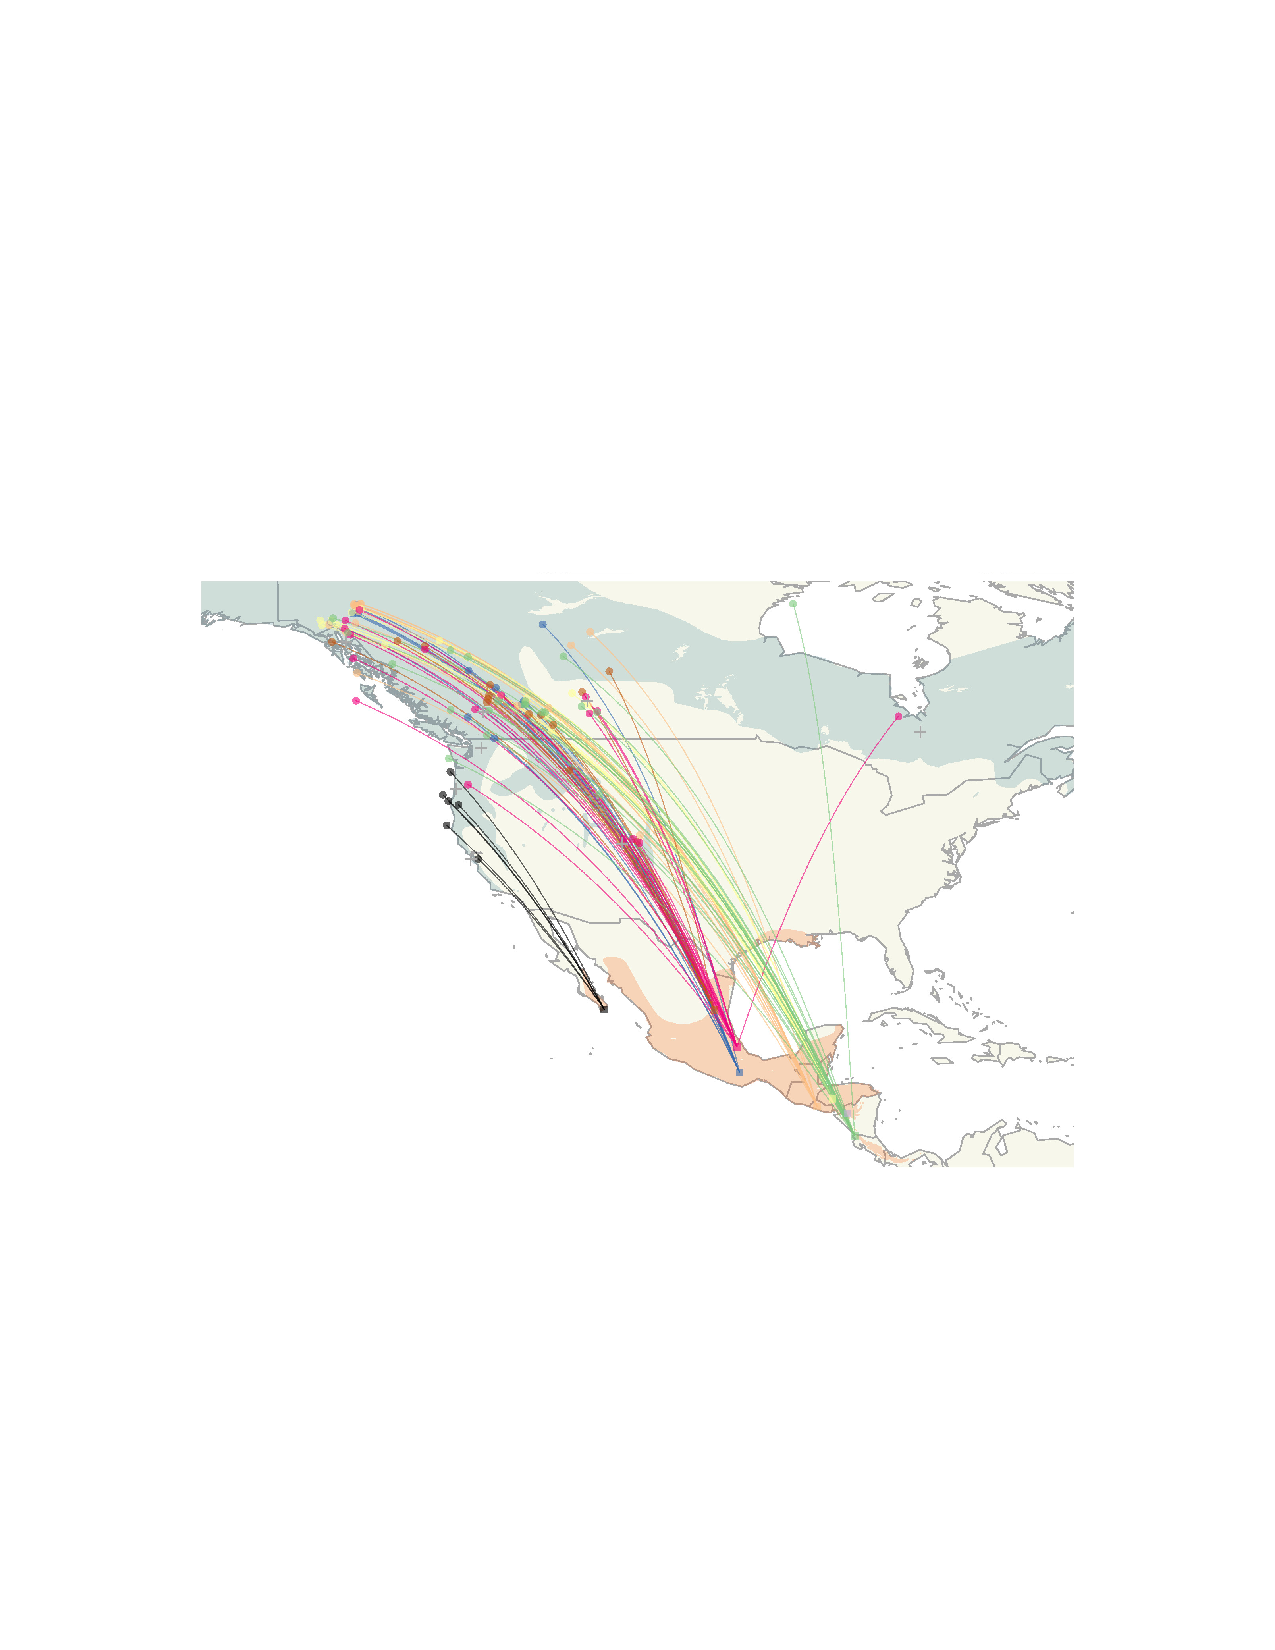
\includegraphics[width=0.9\textwidth]{figs/wintering.pdf}
\end{center}

\end{frame}

\end{document}
